\section{Experiments}
\label{sec:experiments}

Section~\ref{sec:exp-object} isolates the retrieval \emph{object}: every
compared system revises byte-identical frozen forecasts, so any accuracy
difference comes from what is retrieved. Section~\ref{sec:exp-breadth} measures
the resulting revision layer across heterogeneous forecasters, and
Section~\ref{sec:exp-analysis} analyses which correction each deployment picks.

\paragraph{Datasets and backbones.}
Following \citet{liu2025timefuse} and \citet{wang2024lib} we use 16 benchmarks:
ETTh1, ETTh2, ETTm1, ETTm2, Weather, Electricity, and Traffic at horizons
$\{96,192,336,720\}$; PEMS03/04/07/08~\citep{Chen2001FreewayPM} at
$\{6,12,24\}$; and the EPF markets NP, PJM, BE, FR, and
DE~\citep{lago2021epf} at horizon 24. We correct 13 forecasters implemented in
\texttt{TSLib}~\citep{wang2024lib} with their official configurations, L2 loss,
and seed 2021: TimeXer, TimeMixer, PAttn, iTransformer, TimesNet, PatchTST,
DLinear, FreTS, FEDformer, Non-stationary Transformer, LightTS, Informer, and
Autoformer
\citep{wang2024timexer,wang2024timemixer,tan2024pattn,liu2024itransformer,
wu2023timesnet,patchtst,dlinear,yi2024frets,zhou2022fedformer,
Liu2022NonstationaryTR,lightts,zhou2021informer,wu2021autoformer}. Each backbone
is corrected independently, so one dataset--backbone--horizon combination is one
\emph{setting}: 585 in total, comprising 364 long-term, 156 PEMS, and 65 EPF.
Appendix Table~\ref{tab:dataset-scope} gives input lengths and preprocessing.

\paragraph{Protocol.}
A backbone is trained once and never modified. Frozen validation forecasts build
memory, validation labels lock one policy per setting, and that policy is applied
once to test; test labels never enter selection
(Appendix~\ref{app:causality}). Section~\ref{sec:exp-object} additionally
freezes the base predictions, so all six systems revise the same 585 forecast
tensors under one validation split, memory boundary, and scoring rule, with every
search grid frozen before that comparison ran
(Appendix~\ref{app:retrieval-baselines}). Long-term and EPF settings report MSE
and MAE in normalized space, PEMS reports inverse-scaled MAE, RMSE, and MAPE, and
a \emph{strict win} requires every metric a setting reports to decrease. Because
backbone errors span an order of magnitude, we report medians of paired relative
gains alongside means.

\paragraph{Compared retrieval objects.}
\textbf{Analog-kNN} is the input-retrieval control: identical
nearest-neighbour machinery, but it retrieves endpoint-aligned historical
\emph{futures}. \textbf{RAFT}~\citep{han2025raft} and
\textbf{SARAF}~\citep{zhou2026saraf} contribute two published retrieval
operators---RAFT's multiscale endpoint-offset matching and SARAF's
stationarity-controlled relevance--diversity selection---applied to the fixed
forecasts. \textbf{Residual-kNN} is \method{} restricted to its error-retrieval
family, isolating the object change from the gate, and \textbf{\method{}} is the
complete method. Section~\ref{sec:exp-analysis} runs three published systems end
to end in their own protocols.

\subsection{What should a forecaster retrieve?}
\label{sec:exp-object}

% Generated by paper/tools/generate_comparison_tables.py; do not edit.
\begin{table}[t]
\centering
\caption{\textbf{What should a forecaster retrieve?} Every column revises the \emph{same} 585 frozen base forecasts under one validation split, causal memory boundary, and scoring rule; only the retrieved object differs. Lower is better; \bs{1st} and \sbs{2nd} best per column group. PEMS RMSE is in Appendix \ref{app:retrieval-baselines}.}
\label{tab:main-results}
\resizebox{\textwidth}{!}{%
\setlength{\tabcolsep}{3pt}
\begin{tabular}{@{}l|c|c|c|c|c|c@{}}
\toprule
\textbf{Dataset} & \textbf{Frozen} & \multicolumn{3}{c|}{\textbf{Retrieve inputs / futures}} & \multicolumn{2}{c}{\textbf{Retrieve errors (ours)}} \\
\cmidrule(lr){3-5} \cmidrule(lr){6-7}
\textbf{Metrics} & \textbf{Base} & \textbf{Analog-kNN} & \textbf{RAFT} & \textbf{SARAF} & \textbf{Residual-kNN} & \textbf{\method{}} \\
\midrule
\multicolumn{7}{@{}l}{\textit{Long-term, 364 settings (7 datasets, 13 backbones, horizons 96/192/336/720) --- MSE / MAE}} \\
\textbf{ETTh1} & 0.529 0.497 & 0.508 0.487 & 0.502 0.486 & \sbs{0.501} \sbs{0.485} & 0.519 0.494 & \bs{0.479} \bs{0.468} \\
\textbf{ETTh2} & 0.597 0.515 & \bs{0.431} \bs{0.438} & 0.441 0.442 & 0.443 0.444 & 0.544 0.493 & \sbs{0.435} \sbs{0.439} \\
\textbf{ETTm1} & 0.481 0.453 & \sbs{0.442} \sbs{0.437} & 0.455 0.441 & 0.455 0.441 & 0.447 0.440 & \bs{0.423} \bs{0.425} \\
\textbf{ETTm2} & 0.385 0.394 & \sbs{0.295} \sbs{0.344} & 0.305 0.352 & 0.305 0.352 & 0.364 0.383 & \bs{0.292} \bs{0.340} \\
\textbf{Weather} & 0.321 0.338 & \sbs{0.286} \sbs{0.319} & 0.292 0.322 & 0.293 0.323 & 0.289 0.324 & \bs{0.271} \bs{0.308} \\
\textbf{Electricity} & 0.242 0.329 & \bs{0.207} \bs{0.305} & 0.213 0.308 & \sbs{0.212} 0.308 & 0.216 0.310 & 0.213 \sbs{0.307} \\
\textbf{Traffic} & 0.597 0.361 & 0.574 0.354 & 0.579 0.356 & 0.575 0.356 & \bs{0.550} \sbs{0.343} & \sbs{0.557} \bs{0.342} \\
\midrule
\textbf{Long-term average} & 0.450 0.413 & \sbs{0.392} \sbs{0.383} & 0.398 0.387 & 0.398 0.387 & 0.418 0.398 & \bs{0.382} \bs{0.376} \\
\midrule
\multicolumn{7}{@{}l}{\textit{PEMS traffic flow, 156 settings (horizons 6/12/24), inverse-scaled --- MAE / MAPE}} \\
\textbf{PEMS03} & 20.781 0.208 & \bs{17.097} \bs{0.168} & 19.855 0.196 & 19.886 0.196 & 18.224 0.182 & \sbs{18.131} \sbs{0.182} \\
\textbf{PEMS04} & 26.982 0.189 & \bs{22.541} \bs{0.149} & 25.911 0.179 & 25.972 0.180 & \sbs{23.664} \sbs{0.161} & 23.706 0.161 \\
\textbf{PEMS07} & 30.087 0.139 & \bs{24.210} \bs{0.104} & 28.865 0.133 & 28.940 0.133 & 26.224 0.118 & \sbs{26.191} \sbs{0.118} \\
\textbf{PEMS08} & 23.086 0.148 & \bs{18.069} \bs{0.114} & 22.005 0.139 & 22.049 0.139 & \sbs{19.654} 0.127 & 19.854 \sbs{0.127} \\
\midrule
\textbf{PEMS average} & 25.234 0.171 & \bs{20.479} \bs{0.134} & 24.159 0.162 & 24.212 0.162 & \sbs{21.942} 0.147 & 21.970 \sbs{0.147} \\
\midrule
\multicolumn{7}{@{}l}{\textit{EPF electricity price, 65 settings (horizon 24) --- MSE / MAE}} \\
\textbf{NP} & 0.314 0.328 & 0.295 0.311 & \sbs{0.294} 0.311 & \bs{0.291} \bs{0.309} & 0.301 0.320 & 0.294 \sbs{0.310} \\
\textbf{PJM} & 0.121 0.224 & 0.110 0.216 & 0.110 0.216 & \sbs{0.109} 0.216 & 0.114 \sbs{0.216} & \bs{0.107} \bs{0.209} \\
\textbf{BE} & 0.453 0.305 & 0.451 0.296 & 0.447 0.298 & 0.448 0.300 & \sbs{0.425} \sbs{0.294} & \bs{0.421} \bs{0.289} \\
\textbf{FR} & 0.465 0.258 & 0.469 \sbs{0.242} & 0.455 0.248 & 0.457 0.246 & \sbs{0.453} 0.244 & \bs{0.423} \bs{0.237} \\
\textbf{DE} & 0.526 0.459 & 0.506 \bs{0.449} & \sbs{0.506} 0.449 & \bs{0.505} \sbs{0.449} & 0.520 0.451 & 0.515 0.455 \\
\midrule
\textbf{EPF average} & 0.376 0.315 & 0.366 \sbs{0.303} & 0.362 0.304 & \sbs{0.362} 0.304 & 0.363 0.305 & \bs{0.352} \bs{0.300} \\
\bottomrule
\end{tabular}%
}
\end{table}

% Generated by paper/tools/generate_comparison_tables.py; do not edit.
\begin{table}[t]
\centering
\small
\caption{\textbf{Strict wins over the frozen base}, counted only when \emph{every} metric a setting reports decreases. Rows above the rule retrieve inputs and their futures; rows below retrieve model errors. Bold marks the largest count per column.}
\label{tab:retrieval-win-summary}
\setlength{\tabcolsep}{6pt}
\begin{tabular}{@{}lrrrr@{}}
\toprule
System & LT (364) & PEMS (156) & EPF (65) & All (585) \\
\midrule
Analog-kNN & 272/364 & \textbf{156/156} & 50/65 & 478/585 \\
RAFT & 251/364 & 74/156 & 50/65 & 375/585 \\
SARAF & 256/364 & 74/156 & 54/65 & 384/585 \\
\midrule
Residual-kNN & 273/364 & \textbf{156/156} & \textbf{61/65} & 490/585 \\
\method{} & \textbf{325/364} & 155/156 & 53/65 & \textbf{533/585} \\
\bottomrule
\end{tabular}
\end{table}


\begin{figure}[t]
  \centering
  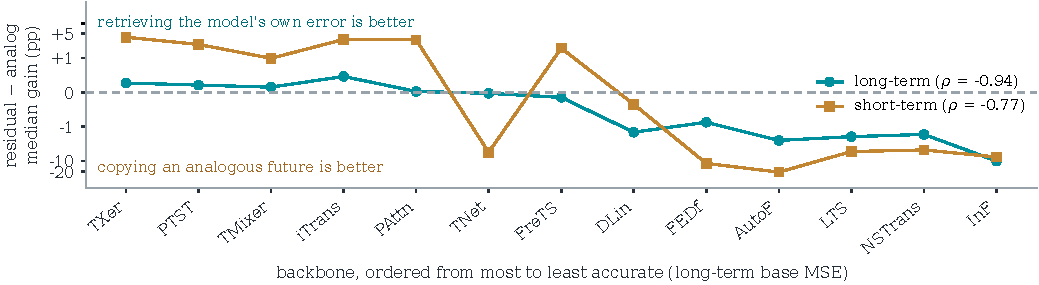
\includegraphics[width=\textwidth]{figures/retrieval_object_vs_strength.pdf}
  \caption{\textbf{The better retrieval object depends on how good the frozen
  forecaster already is.} Each point is the median, over one backbone's settings
  in one family, of the smallest paired relative gain across that setting's
  metrics; the curve plots Residual-kNN minus Analog-kNN in percentage points on a
  symmetric-log axis, with backbones ordered from most to least accurate by mean
  long-term base MSE. For the five most accurate backbones, retrieving the
  forecaster's own error wins on long-term and PEMS settings.}
  \label{fig:object-strength}
\end{figure}

\paragraph{Absolute accuracy.}
In Table~\ref{tab:main-results}, \method{} takes the lowest long-term average,
0.382/0.376 against 0.450/0.413 for the frozen base, winning both metrics on four
of seven datasets and coming within 0.007 of the best on the other three; it also
takes the best EPF average, 0.352/0.300 against 0.376/0.315. Two aggregates
favour the future object, long-term (0.392/0.383 against 0.418/0.398) and PEMS
MAE (20.479 against 21.942), and both are set by the weakest backbones: Informer
alone has a base MSE of 1.053, three times the best backbone's, and copying an
aligned analogue repairs a badly wrong trajectory. Excluding Informer, the
median long-term paired reduction favours the error object on both metrics,
2.09\%/0.99\% against 1.97\%/0.66\%. PEMS is the one family where an
endpoint-aligned analogue is already a good forecast, since its traffic flow is
strongly and stably periodic with matched levels across weeks; even there,
Residual-kNN beats Analog-kNN for all five of the most accurate forecasters
(Figure~\ref{fig:object-strength}).

\paragraph{Reliability separates the objects more sharply than accuracy.}
Table~\ref{tab:retrieval-win-summary} counts settings in which \emph{all}
reported metrics improve. Retrieving errors is the most reliable single object,
with 490/585 strict wins against 478 for Analog-kNN and 375 and 384 for RAFT and
SARAF; the full \method{} policy reaches 533/585. The margin over published
operators is largest where it matters: their median paired PEMS reductions are
0.00\% RMSE and 0.36\%/0.31\% MAPE, against 10.24\% RMSE and 12.48\% MAPE for
\method{}, because multiscale input matching returns neighbourhoods dominated by
the traffic profile the backbone already predicts. The retrieval object, not the
retrieval machinery, is the binding design decision.

\paragraph{The right object depends on how strong the forecaster is.}
Figure~\ref{fig:object-strength} explains why the two views disagree. Ordering
the 13 backbones by long-term base MSE, the advantage of retrieving errors over
retrieving futures falls monotonically as base error rises: Spearman $\rho$
between base MSE and that advantage is $-0.94$ on long-term settings, $-0.70$ on
PEMS, and $-0.27$ on EPF. The mechanism is direct. A weak forecaster's prediction
holds little level, phase, or rhythm worth protecting, so overwriting it with an
analogous future is an improvement; an accurate forecaster's prediction already
holds all of that, so overwriting it destroys correct structure and only the
residual is worth transferring. Restricted to the five most accurate
backbones---the regime a practitioner deploys---the error object also wins on
strict counts: 170/225 for Residual-kNN and 185/225 for \method{}, against
157/225 for Analog-kNN and 77/225 and 80/225 for RAFT and SARAF.

\subsection{Correcting 13 heterogeneous frozen forecasters}
\label{sec:exp-breadth}

On the separate primary matrix, where each backbone is trained and corrected end
to end rather than replayed from fixed tensors, \method{} improves every reported
metric in 562/585 settings (96.1\%): 355/364 long-term, 151/156 PEMS, and 56/65
EPF. Mean paired reductions are 8.5\% MSE, 7.5\% MAE, 10.6\% RMSE, and 12.0\% MAPE.
Appendix Table~\ref{tab:backbone-results} shows no backbone left behind: all 13
improve on at least 25 of their 28 long-term settings, and on 12 of 12 PEMS
settings for every backbone but TimeMixer. Gains scale with how much error there
is to remove, from 1.1\% long-term MSE for TimeXer to 41.3\% for Informer, as an
additive layer that leaves a good forecast alone should. The selection rule and margin were designed on a predetermined 123-setting
development subset and then frozen; on the 462 held-out settings the strict-win
rate is 437/462 (94.6\%) and every pre-registered criterion still passes
(Appendix~\ref{app:aggregate-results}). An independent replication on different
hardware reproduces 581/585 strict-win decisions.

\paragraph{Error retrieval transfers to ensembles, AutoML, and foundation
models.}
Because \method{} consumes only predictions and targets, one interface covers
systems that are not single neural networks: greedy forward
selection~\citep{caruana2004ensemble}, a portfolio and a zero-shot
ensemble~\citep{autosklearn_portfolio_zeroshot}, AutoGluon's
\texttt{high\_quality} predictor~\citep{shchur2023autogluon}, and Chronos-Bolt in
fine-tuned and zero-shot form~\citep{ansari2024chronos}.
Appendix Table~\ref{tab:strong-systems} reports 81/94 strict wins (86.2\%): 33/40
long-term, 24/24 PEMS, and 24/30 EPF, with per-system rates from 12/16 for the
portfolio ensemble to 16/16 for zero-shot Chronos-Bolt. This is also the
strongest direct evidence for error retrieval, since validation selects the
residual family in 70 of the 94 settings and 65 of those are strict wins.
Systems assembled from many components, and a foundation model applied off its
pretraining distribution, leave error structure their own machinery does not
remove.

\subsection{Analysis}
\label{sec:exp-analysis}

\paragraph{Which correction wins is a property of the deployment.}
Across the primary matrix, validation selects error retrieval in 214/585
settings, seasonal blending in 156, overlap blending in 159, and causal bias in
56. The composition swings with the backbone, from 29/45 settings for DLinear to
5/45 for Informer, and with the dataset, from 35/39 for PEMS03 to 0/52 for ETTh2
(Appendix Figure~\ref{fig:selection}). The retrieval family delivers 207 of the
562 strict wins and the simpler corrections the remaining 355. Error retrieval is
therefore the largest single contributor and the object a retrieval layer should
default to, while the gate keeps that default from firing where a temporal
correction is the honest answer.

\paragraph{Published retrieval systems on their own bases.}
We also run three published retrieval-augmented forecasters end to end, each
paired with its released no-retrieval base under its own protocol.
RAF~\citep{tire2024raf} improves both reported metrics in 33/44 paired
configurations and TS-RAG~\citep{ning2025tsrag} in 7/7, whereas
RATD~\citep{liu2024ratd} degrades its CSDI base on its single Electricity pair,
RMSE $0.3891\!\rightarrow\!0.6374$. Retrieval augmentation is useful but not
automatically safe even natively---hence the gate of
Section~\ref{sec:selection}.

\paragraph{Corrections keep working on later observations.}
A frozen correction is useful only if it survives the passage of time. We replay
TimeMixer checkpoints at horizon 96 on the four ETT datasets for seeds 2021--2023
over a timeline beginning after the standard test split, with checkpoints,
scalers, and correction parameters held fixed and labels released only as their
target intervals elapse. Every dataset and seed improves both metrics, with pooled
MSE reductions of 2.10\% to 4.51\% and every paired bootstrap interval below zero
(Appendix~\ref{app:ett}).

\paragraph{Where the revision layer fails.}
Of the 23 settings that are not strict wins, 11 selected overlap blending, seven
error retrieval, and five seasonal blending, and 14 degrade every metric.
Failures concentrate: Weather and EPF-DE account for 14 of them and TimeMixer for
seven, including all five PEMS failures, and the largest single regression is
36.5\% MAPE on a PEMS04 overlap selection. Effect sizes vary too: among the 562
strict wins, at least one metric improves by no more than one percentage point in
120 settings, which is why we report absolute values and continuous gains
alongside counts.
